\begin{frame}{Generative World Models: Sora}
  \begin{columns}[T,onlytextwidth]
    \column{0.48\textwidth}
    \begin{itemize}\footnotesize
      \item Generates high-quality, minute-long videos with strong visual coherence for a wide range of physical and digital scenes.
      \item Rapidly turns text prompts into compelling videos, accelerating creative work, education, and accessibility.
      \item Enables new applications in marketing, game development, and more through scalable video generation.
    \end{itemize}
    \column{0.50\textwidth}
    \centering
    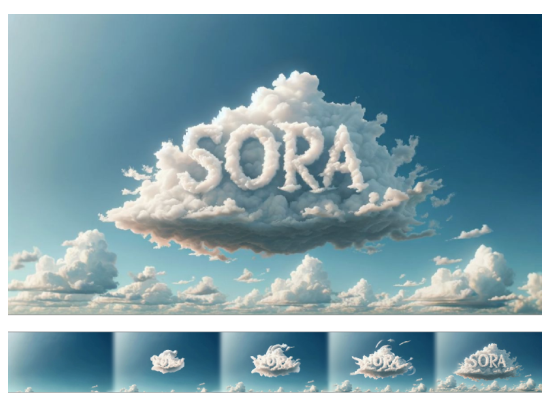
\includegraphics[width=\linewidth,height=0.70\textheight,keepaspectratio]{assets/New-Lecture-Video_Generation/sora_arxiv2402177_p01_fig1_title.png}\\[-0.12em]
    {\scriptsize Liu et al.\ (2024); \href{https://arxiv.org/abs/2402.17177}{arXiv:2402.17177}}
  \end{columns}
\end{frame}

% ----- OpenAI Sora (Liu et al. survey, arXiv:2402.17177) -----
\begin{frame}{A Brief History: From Texture Synthesis to Sora}
  \centering
  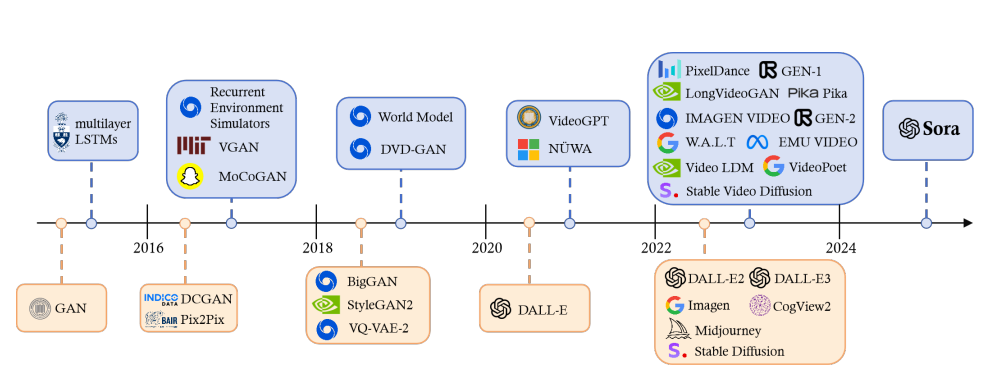
\includegraphics[width=\linewidth,height=0.56\textheight,keepaspectratio]{assets/New-Lecture-Video_Generation/genai_vision_history.png}
  \footnotesize
  \begin{itemize}\footnotesize
    \item \textbf{Before deep learning:} Image generation relies on hand-crafted features.
    \item \textbf{The deep learning revolution:} GANs and VAEs brought greater realism in images, diffusion models become backbone of modern visual generation.
    \item \textbf{Transformers and modality fusion:} Transformers, adapted from NLP (BERT, GPT) to vision tasks (e.g.\ ViT), enable new capabilities; multimodal models (e.g. CLIP) align vision and language for T2I and T2V generation.
    \item \textbf{Sora and beyond:} Models like Sora represent the frontier---generating high-quality, minute-long videos from text prompts.
  \end{itemize}
\end{frame}

\begin{frame}[t,allowframebreaks]{Sora Core: Diffusion Transformer Architecture}
  \centering
  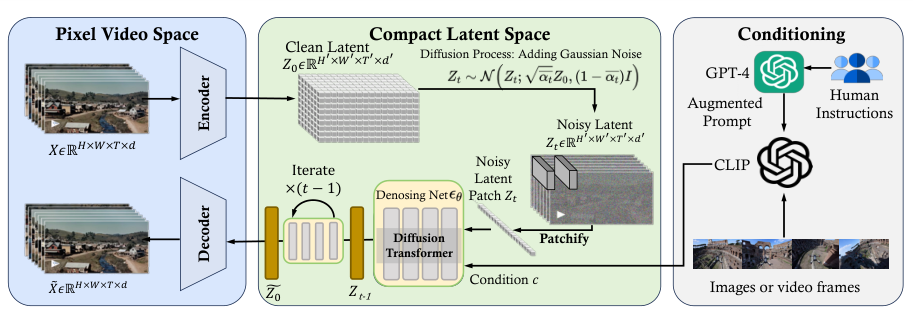
\includegraphics[width=\linewidth,height=0.78\textheight,keepaspectratio]{assets/New-Lecture-Video_Generation/sora_arxiv2402177_p06_fig4_framework.png}\\[0.12em]
  \begin{itemize}\footnotesize
    \item Time-space compressor: compresses input video into compact latent space representation.
    \item ViT processes tokenized latents and predicts denoised versions.
    \item CLIP-like conditioning: incorporates user instructions and visual prompts, guiding generation with learned theme and style.
    \item Denoising and decoding: after multiple denoising steps, final latent video decoded back into pixel space to yield generated video.
  \end{itemize}
\end{frame}

\begin{frame}{Sora: Limitations}
  \begin{itemize}\itemsep0.26em
    \item \textbf{Physical realism:} unstable causal detail (e.g.\ objects not updating consistently after contact); implausible rigid-body motion; occasional absurd multi-object interactions.
    \item \textbf{Spatial/temporal control:} confusion over placement and left/right; drift in camera motion and event order; stray characters or animals that break the intended shot.
    \item \textbf{Interaction \& prompting:} fine-grained local edits remain difficult; complex natural-language constraints may be misread.
    \item \textbf{Access:} no fixed public release schedule at review time---safety and readiness framing ({OpenAI}).
  \end{itemize}
\end{frame}
